\documentclass[10pt]{memoir}
\setstocksize{220mm}{155mm} 	        
\settrimmedsize{220mm}{155mm}{*}	
\settypeblocksize{170mm}{116mm}{*}	
\setlrmargins{18mm}{*}{*}
\setulmargins{*}{*}{1.2}
%\setlength{\headheight}{5pt}%
\checkandfixthelayout[lines]
\linespread{1.16}
\flushbottom

%%% Hyphenation settings
\usepackage[htt]{hyphenat}
\hyphenation{he-lio-trope opos-sum}
\tracingparagraphs=1
%Hyphenation in Devanāgarī of the edition still missing? Probably this needs to be modified in babel-iast package? 

%%% babel
\usepackage[english]{babel}
\usepackage{babel-iast/babel-iast}

\babelfont[iast]{rm}[Renderer=Harfbuzz, Scale=1.3]{AdishilaSan}%AdishilaSan}
\babelfont[english]{rm}{Adobe Text Pro}

%%% more functionality
\PassOptionsToPackage{hyphens}{url}
\usepackage{hyperref}
\usepackage{pdflscape}
\usepackage{cleveref}
\usepackage{url}
\usepackage{cleveref}
\usepackage{microtype}
\usepackage{lineno}

%\usepackage{bigfoot}
%%% more functions
\usepackage[dvipsnames]{xcolor}
%\usepackage[para,perpage]{footmisc}

%%%für den Counter von Kapiteln und Sätzen! 
\newcommand{\uproman}[1]{\uppercase\expandafter{\romannumeral#1}}
\newcommand{\lowroman}[1]{\romannumeral#1\relax}

\makeindex
\newfontfamily\sanskritfont[Script=Devanagari,Mapping=RomDev,Scale=1.1]{Sanskrit2003}
\usepackage{pifont,fourier-orns,lettrine,psvectorian,paralist,enumitem,pdfpages,wrapfig,tabulary,lettrine,longtable}
\setlist[enumerate]{itemsep=0mm}
\usepackage[autostyle]{csquotes}
\usepackage[defaultlines=2,all]{nowidow}
\usepackage{ellipsis,adforn,booktabs,longtable,url,tikz}
\lineskiplimit=-3pt          

\makechapterstyle{IeT}{%
  \chapterstyle{default}
  \renewcommand*{\printchapternonum}{\centering}
  \renewcommand*{\clearforchapter}{\cleartorecto} 
  \aliaspagestyle{chapter}{empty}}
\chapterstyle{IeT}
\setsecnumdepth{none}  \openright  \nouppercaseheads
\settocdepth{subsubsection}

%%%% test better pagebreaks
%\def\fussy{%
%  \emergencystretch\z@
%  \tolerance 200%
%  \hfuzz .1\p@
%  \vfuzz\hfuzz}

%\interfootnotelinepenalty=10000\relax

%\usepackage[maxfloats=256]{morefloats}

%\maxdeadcycles=500

%raggedbottomsectiontrue
%%\checkandfixthelayout


%%%%%%%  biblatex
%\newcommand{\noun}[1]{\textsc{#1}}    %  philosophy-verbose
\usepackage[backend=biber, sorting=nyt, style=verbose]{biblatex} %%%%ORIGINAL TiE
\renewcommand*{\mkbibnamefamily}[1]{\textsc{#1}}


\DeclareFieldFormat{url}{%
  \mkbibacro{URL}\addcolon\space
  \href{#1}{\nolinkurl{\thefield{urlraw}}}}

\DeclareFieldFormat{citeurl}{%
  \href{#1}{\nolinkurl{\thefield{urlraw}}}} 


\DeclareFieldFormat{postnote}{#1}
\renewcommand{\postnotedelim}{, }
\addbibresource{bindu.bib}

%%% ekdosis
\usepackage[teiexport=tidy,parnotes=true]{ekdosis}% =tidy cleans up HTML and XML documents by fixing markup errors and upgrading legacy code to modern standards. parnotes=footnotes below or above critical apparatus

\SetLineation{lineation=page, modulo} %lineation=page sets thenumbering to start afresh at the top of each page. =modulo makes every fifth line numbered. {lineation=page} makes every line numbered! 

\renewcommand{\linenumberfont}{\selectlanguage{english}\footnotesize} %sets language of lines to English

\SetTEIxmlExport{autopar=false} %autopar=falseinstructs ekdosis to ignore blank lines in the.tex sourcefile as markers for paragraph boundaries. As a result, each paragraph of the edition must be found within an environment associated with the xml <p> element

\SetHooks{
  lemmastyle=\bfseries,
  %refnumstyle=\selectlanguage{english}\bfseries,
  refnumstyle=\selectlanguage{english}\color{blue}\bfseries,
  appheight=0.8\textheight,
}

\newif\ifinapparatus
\DeclareApparatus{source}[
%bhook=\inapparatustrue,
lang=english,
notelang=english,
% bhook=\selectlanguage{english},
bhook=\selectlanguage{english}\textbf{Sources:},%
%maxentries=4, 
%ehook=.]
%sep={] },
%nosep,
]

\newif\ifinapparatus
\DeclareApparatus{testium}[
%bhook=\inapparatustrue,
lang=english,
notelang=english,
% bhook=\selectlanguage{english},
bhook=\selectlanguage{english}\textbf{Testimonia:},
%maxentries=4, 
%ehook=.]
%nosep, 
]

% Declare \ifinapparatus and set \inapparatustrue at the beginning of
% the apparatus criticus block. Also set the language.  
\newif\ifinapparatus
  \DeclareApparatus{default}[
  %bhook=\inapparatustrue, 
  lang=english,
  %maxentries=33,
  %bhook=\selectlanguage{english},
  sep = {] },
  delim=\hskip 0.75em,
  rule=\rule{0.7in}{0.4pt},
]

\newif\ifinapparatus
\DeclareApparatus{philcomm}[
%bhook=\inapparatustrue,
lang=english,
notelang=english,
bhook=\selectlanguage{english}\textbf{Philological Commentary:},
%bhook=\selectlanguage{english},
sep={: },
]

\ekdsetup{
showpagebreaks,
spbmk = \textcolor{blue}{spb},
hpbmk = \textcolor{red}{hpb}
}

%\usepackage{fnpos}
%\makeFNmid
%\makeFNbottom
\usepackage[bottom]{footmisc}
%%%%%%%%%%%%%%%%%%%%%%%%%%%
\makeatletter
\def\blfootnote{\gdef\@thefnmark{}\@footnotetext}
\makeatother
%%%%%%%%%%%%%%%%%%%%%%%%%


% Macros and Definitions for the Print of Sigla
\def\acpc#1#2#3{{#1}\rlap{\textrm{\textsuperscript{#3}}}\textsubscript{\textrm{#2}}\space}
\def\sigl#1#2{{{#1}}\textsubscript{\textrm{#2}}}
\def\None{{\sigl{N}{1}}} \def\Noneac{\acpc{N}{1}{ac}\,} \def\Nonepc{\acpc{N}{1}{pc}\,}
\def\Ntwo{{\sigl{N}{2}}} \def\Noneac{\acpc{N}{2}{ac}\,} \def\Nonepc{\acpc{N}{2}{pc}\,}
\def\Done{{\sigl{D}{1}}} \def\Doneac{\acpc{D}{1}{ac}\,} \def\Donepc{\acpc{D}{1}{pc}\,}
\def\Dtwo{{\sigl{D}{2}}} \def\Dtwoac{\acpc{D}{2}{ac}\,} \def\Dtwopc{\acpc{D}{2}{pc}\,}
\def\Uone{{\sigl{U}{1}}} \def\Uoneac{\acpc{U}{1}{ac}\,} \def\Uonepc{\acpc{U}{1}{pc}\,}                 
\def\Utwo{{\sigl{U}{2}}} \def\Utwoac{\acpc{U}{2}{ac}\,} \def\Utwopc{\acpc{U}{2}{pc}\,}

%%%%%%%%%%%%%% Tattvabinduyoga - List of Witnesses   %%%%%%%%%%%%%%%%%%%
\DeclareWitness{ceteri}{\selectlanguage{english}cett.}{ceteri}[]   
\DeclareWitness{E}{\selectlanguage{english}E}{Printed Edition}[]    
\DeclareWitness{P}{\selectlanguage{english}P}{Pune BORI 664}[]  
\DeclareWitness{B}{\selectlanguage{english}B}{Bodleian 485}[]       
\DeclareWitness{N1}{\selectlanguage{english}N\textsubscript{1}}{NGMPP 38/31}[]
\DeclareWitness{N2}{\selectlanguage{english}N\textsubscript{2}}{NGMPP B 38/35}[]
\DeclareWitness{L}{\selectlanguage{english}L}{LALCHAND 5876}[]  
\DeclareWitness{D}{\selectlanguage{english}D}{IGNCA 30019}[] 
%\DeclareWitness{D2}{\selectlanguage{english}D\textsubscript{2}}{IGNCA 30020}[]  
\DeclareWitness{U1}{\selectlanguage{english}U\textsubscript{1}}{SORI 1574}[] 
\DeclareWitness{U2}{\selectlanguage{english}U\textsubscript{2}}{SORI 6082}[]
%%%%%%%%%%%%%% Tattvabinduyoga - Groups of Witnesses   %%%%%%%%%%%%%%%%%%%
\DeclareWitness{X}{\selectlanguage{english}\alpha}{Alpha Group: D,N1,N2,U1}[]
\DeclareWitness{Y}{\selectlanguage{english}\beta}{Beta Group: B,E,L,P,U2}[]
%%%%%%%%%%%%% Testimonia
\DeclareWitness{Ysv}{\selectlanguage{english}Ysv}{Yogasvarodaya}[] %%%add infos!  

%%%%%%%%%%%%%%%%%%%%%%%%%%%%%%%%%%%%%%%%%%%
% Macro for Editing Abbrevs.
\def\om{\textrm{\footnotesize \textit{om.}\ }} %prints om. for omitted in apparatus
\def\korr{\textrm{\footnotesize \textit{em.}\ }} %prints em. for emended in apparatus
\def\conj{\textrm{\footnotesize \textit{conj.}\ }} %prints conj. for conjectured in apparatus

% \supplied{text} EDITORIAL ADDITION -> Within \lem oder \rdg
% \surplus{text} EDITORIAL DELETION -> Within \lem oder \rdg
% \sic{text} CRUX
% \gap{text} LACUNAE -> [reason=??, unit=??, quantity=??, extent=??]


%%%%%%%%%%%%%%%%%%%%%%%%%%%%%%%%%%%%%%%%%%% All macros of this list can be used in 
% Macro for Editing Abbrevs.
\def\eyeskip{\textrm{{ab.\,oc. }}}
\def\aberratio{\textrm{{ab.\,oc. }}}
\def\ad{\textrm{{ad}}}
\def\add{\textrm{{add.\ }}}
\def\ann{\textrm{{ann.\ }}}
\def\ante{\textrm{{ante }}} 
\def\post{\textrm{{post }}}
%\def\ceteri{cett.\,}                   
\def\codd{\textrm{{codd.\ }}}

\def\coni{\textrm{{coni.\ }}}
\def\contin{\textrm{{contin.\ }}}
\def\corr{\textrm{{corr.\ }}}
\def\del{\textrm{{del.\ }}}
\def\dub{\textrm{{ dub.\ }}}

\def\expl{\textrm{{explic.\ }}} 
\def\explica t{\textrm{{explic.\ }}}
\def\fol{\textrm{{fol.\ }}}
\def\foll{\textrm{{foll.\ }}}
\def\gloss{\textrm{{glossa ad }}}
\def\ins{\textrm{{ins.\ }}}      
\def\inseruit{\textrm{{ins.\ }}} 
\def\im{{\kern-.7pt\lower-1ex\hbox{\textrm{\tiny{\emph{i.m.}}}\kern0pt}}} %\textrm{\scriptsize{i.m.\ }}}      
\def\inmargine{{\kern-.7pt\lower-.7ex\hbox{\textrm{\tiny{\emph{i.m.}}}\kern0pt}}}%\textrm{\scriptsize{i.m.\ }}}      
\def\intextu{{\kern-.7pt\lower-.95ex\hbox{\textrm{\tiny{\emph{i.t.}}}\kern0pt}}}%\textrm{\scriptsize{i.t.\ }}}           
\def\indist{\textrm{{indis.\ }}}  
\def\indis{\textrm{{indis.\ }}}
\def\iteravit{\textrm{{iter.\ }}} 
\def\iter{\textrm{{iter.\ }}}
\def\lectio{\textrm{{lect.\ }}}   
\def\lec{\textrm{{lect.\ }}}
\def\leginequit{\textrm{{l.n. }}} 
\def\legn{\textrm{{l.n. }}}
\def\illeg{\textrm{{l.n. }}}

\def\primman{\textrm{{pr.m.}}}
\def\prob{\textrm{{prob.}}}
\def\rep{\textrm{{repetitio }}}
\def\secundamanu{\textrm{\scriptsize{s.m.}}}            \def\secm{{\kern-.6pt\lower-.91ex\hbox{\textrm{\tiny{\emph{s.m.}}}\kern0pt}}}%   \textrm{\scriptsize{s.m.}}}
\def\sequentia{\textrm{{seq.\,inv.\ }}}  
\def\seqinv{\textrm{{seq.\,inv.\ }}}
\def\order{\textrm{{seq.\,inv.\ }}}
\def\supralineam{{\kern-.7pt\lower-.91ex\hbox{\textrm{\tiny{\emph{s.l.}}}\kern0pt}}} %\textrm{\scriptsize{s.l.}}}
\def\interlineam{{\kern-.7pt\lower-.91ex\hbox{\textrm{\tiny{\emph{s.l.}}}\kern0pt}}}   %\textrm{\scriptsize{s.l.}}}
\def\vl{\textrm{v.l.}}   \def\varlec{\textrm{v.l.}} \def\varialectio{\textrm{v.l.}}
\def\vide{\textrm{{cf.\ }}}
\def\cf{\textrm{{cf.\ }}} 
\def\videtur{\textrm{{vid.\,ut}}}
\def\crux{\textup{[\ldots]} }
\def\cruxx{\textup{[\ldots]}}
\def\unm{\textit{unm.}}
%%%%%%%%%%%%%%%%%%%%%%%%%%%%%%%%%%%%

% List of Scholars
\DeclareScholar{ego}{ego}[
forename=Nils Jacob,
surname=Liersch]

% Persons:14\DeclareScholar{ego}{ego}[15forename=Robert,16surname=Alessi]17% Useful shorthands:18\DeclareShorthand{codd}{codd.}{V,I,R,H}19\DeclareShorthand{edd}{edd.}{Lit,Erm,Sm}20\DeclareShorthand{egoscr}{\emph{scripsi}}{ego}

%Useful shorthands:
%\DeclareShorthand{codd}{codd.}{V,I,R,H}
%\DeclareShorthand{edd}{edd.}{Lit,Erm,Sm}
\DeclareShorthand{egoscr}{em.}{ego}
\DeclareShorthand{egoscrconj}{conj.}{ego}
\DeclareShorthand{egomute}{\unskip}{ego}

\usepackage{xparse}

\NewDocumentEnvironment{tlg}{O{}O{}}{\setlength{\leftskip}{0pt}\vspace{-1ex}\begin{quotation}}{\hfill #1\ \vspace{-1ex}\end{quotation}\vspace{-1ex}} %verse environment
%\NewDocumentEnvironment{tlg}{O{}O{}}{\begin{verse}}{॥#1\hskip-4pt ॥\\ \end{verse}}
\NewDocumentCommand{\tl}{m}{{\selectlanguage{iast} #1}}

\NewDocumentCommand{\extra}{m}{{\textcolor{gray}{#1}}} %command for additions to U2
\NewDocumentCommand{\crazy}{m}{{\textcolor{red}{#1}}} %totally corrupted passage
\NewDocumentCommand{\coro}{m}{{\textcolor{violet}{#1}}} %colour for sentence counter! 

\NewDocumentEnvironment{prose}{O{}}{\begin{otherlanguage}{iast}}{\end{otherlanguage}}
% \NewDocumentEnvironment{padd}{O{}}{\begin{otherlanguage}{iast}}{\end{otherlanguage}}
\NewDocumentEnvironment{tlate}{O{}}
%\NewDocumentEnvironment{tadd}{O{}}

%Define two commands: \skp ("sanskrit plus"), to be ignored by TeX in
%the edition text, but processed in the TEI output. Conversely, \skm
%("sanskrit minus") is to be processed in the edition text, but
%ignored if found in the apparatus criticus and in the TEI output:

\NewDocumentCommand{\skp}{m}{}
\TeXtoTEIPat{\skp {#1}}{#1}

%\NewDocumentCommand{\skpp}{m}{}
%\TeXtoTEIPat{\skpp {#1}}{#1}

\NewDocumentCommand{\skm}{m}{\unless\ifinapparatus#1-\fi}
\TeXtoTEIPat{\skm {#1}}{}

% \NewDocumentCommand{\dd}{}{/\hskip-4pt/}
\NewDocumentCommand{\dd}{}{\mbox{/\hskip-4pt/}}
\TeXtoTEIPat{\dd {}}{//}


%%% modify environments and commands
%%% TEI mapping
\TeXtoTEIPat{\begin {tlg}}{<lg>} %lg=(Group of verse (s)) contains one or more verses or lines of verse that together form a formal unit (e.g. stanza, chorus).
\TeXtoTEIPat{\end {tlg}}{</lg>}

\TeXtoTEIPat{\begin {prose}}{<p>}
\TeXtoTEIPat{\end {prose}}{</p>}

\TeXtoTEIPat{\begin {tlate}}{<p>}
\TeXtoTEIPat{\end {tlate}}{</p>}

\TeXtoTEIPat{\\}{}
\TeXtoTEIPat{\linebreak}{<br/>}
\TeXtoTEIPat{\noindent}{}
%\TeXtoTEI{tl}{l}
\TeXtoTEI{emph}{hi}
\TeXtoTEI{bigskip}{}
\TeXtoTEI{None}{N1}
\TeXtoTEI{Ntwo}{N2}
\TeXtoTEI{Done}{D1}
\TeXtoTEI{Dtwo}{D2}
\TeXtoTEI{Uone}{U1}
\TeXtoTEI{Utwo}{U2}
%\TeXtoTEIPat{/}{ |}
%\TeXtoTEI{//}{ ||}
\TeXtoTEIPat{\korr}{em. }
\TeXtoTEIPat{\conj}{conj.}
\TeXtoTEIPat{\om}{om.}
\TeXtoTEIPat{english}{}
\TeXtoTEIPat{\hskip}{}
\TeXtoTEIPat{\hskip-4pt}{}
\TeXtoTEIPat{\hskip-2pt}{}
\TeXtoTEIPat{-}{ }
\TeXtoTEIPat{4pt}{}
\TeXtoTEIPat{2pt}{}
\TeXtoTEIPat{\textcolor {#1}{#2}}{<hi rend="#1">#2</hi>} 

% Nullify \selectlanguage in TEI as it has been used in
% \DeclareWitness but should be ignored in TEI.
\TeXtoTEI{selectlanguage}{}



\FormatDiv{1}{\begin{center}\Large}{\end{center}}
\FormatDiv{2}{\begin{center}\small}{\end{center}}
\FormatDiv{3}{\bfseries}{.}
\title{Yogatattvabindu of Rāmacandra\\ A Critical Edition and Annotated Translation}
\date{\today}

\parindent=15pt
\begin{document}

% Zitiermöglichkeiten:
%\footcite[See][p.\,1]{goldstein01:_tibet_englis_diction_moder_tibet}
%\footnote{\cite{goldstein01:_tibet_englis_diction_moder_tibet}.}

\frontmatter
\thispagestyle{empty}
\begin{center}
  {\Large \emph{The Yogatattvabindu}}\\[3mm]
\end{center}



\newpage

\

\thispagestyle{empty}



\normalsize


\newpage


\begin{center}
\thispagestyle{empty}

\

\vskip 2mm

\begin{otherlanguage}{iast}
\LARGE \sanskritfont{Yogatattvabindu}
\end{otherlanguage}

\vskip .4cm

\Huge Yogatattvabindu \\[7mm]
\Large Critical Edition\\
with annotated Translation


\large

\vspace{3cm}

Von

Nils Jacob Liersch
\small
\vfill

\vfill

Indica et Tibetica Verlag \\ % $\cdot$ 
Marburg 2024

\vskip 6mm

\end{center}

\newpage
\newpage \ \thispagestyle{empty}
\small  \

\noindent

\
\vfill


\small
\noindent \textbf{Bibliographische Information Der Deutschen Bibliothek}

\noindent
Die Deutsche Bibliothek verzeichnet diese Publikation in der Deutschen Nationalbibliographie;
detaillierte bibliographische Informationen sind im Internet über http://dnb.ddb.de abrufbar.

\noindent
\textbf{Bibliographic information published by Die Deutschen Bibliothek}

\noindent
Die Deutsche Bibliothek lists this publication in the Deutsche Nationalbibliographie; detailed
bibliographic data is available in the Internet at http://dnb.ddb.de.  


\vskip 1cm

\noindent
\copyright\ Indica et Tibetica Verlag, Marburg 2024

\medskip

\noindent
Alle Rechte vorbehalten / All rights reserved

\medskip

\noindent
Ohne ausdrückliche Genehmigung des Verlages ist es nicht gestattet, das Werk oder einzelne Teile
daraus nachzudrucken, zu vervielfältigen oder auf Datenträger zu speichern.

\smallskip

\noindent
Apart from any fair dealing for the purpose of private study, research, criticism or review, no
part of this book may be reproduced or translated in any form, by print, photo form, microfilm, or
any other means without written permission. Enquiries should be made to the publishers.

\bigskip

\noindent
Satz: \ \ Nils Jacob Liersch \\
Herstellung: \ \ BoD – Books on Demand GmbH, Norderstedt  \\

\bigskip

\noindent
%\ISBN     

\normalsize

\newpage

%\maketitle
\clearpage
\tableofcontents
\addtocounter{page}{-1}
\thispagestyle{empty}
\clearpage


\mainmatter

\chapter{Conventions in the Critical Apparatus}
\section{Sigla in the Critical Apparatus}

\begin{itemize}
\item E : Printed Edition
\item P : Pune BORI 664
\item L : Lalchand Research Library LRL5876
\item B : Bodleian Oxford D 4587
\item \None : NGMPP B 38-31
\item \Ntwo : NGMPP B 38-35 / A 1327-14
\item \Done : IGNCA 30019
\item \Uone : SORI 1574
\item \Utwo: SORI 6082
\end{itemize}

\chapter{Critical Edition \& Annotated Translation}
\cleardoublepage
\begin{alignment}[
  texts=edition[class="edition"];
  translation[class="translation"],
  ]
  \begin{edition}
    \ekddiv{
      head={[\uproman{19}. \textbf{haṭhayogaḥ}]},
      type=section,
      depth=2, 
      n=XIV
    }
    \xmlhead[h19]{[XIX. haṭhayogaḥ]}
\label{hathayoga}
    \begin{prose}[p19_01]
      \noindent
%------------------------------
%idānīṃ grahayogaḥ kathyate/  \E %[p.23]
%idānīṃ haṭhayogaḥ kathyate   \P
%idānīṃ haṭhayogaḥ kathyate/  \L
%idānīṃ haṭayoga   kathyate/  \B
%idānīṃ haṭhayogaḥ kathyate//  \N1
%idānīṃ haṭhayogaḥ kathyate/  \D
%idānīṃ haṭhayoga  kathyate// \N2
%idānīṃ haṭhayogaḥ kathyate   \U1
%idānīṃ haṭhayoga  kathyate   \U2
%------------------------------
%Now \textit{haṭhayoga} is explained. 
%------------------------------
idānīṃ
\app{\lem[wit={D,L,P,N1,U1}]{haṭhayogaḥ}
     \rdg[wit={B}]{haṭayoga}
     \rdg[wit={E}]{grahayogaḥ}
     \rdg[wit={U2}]{haṭhayoga}} kathyate/
\note[type=source, labelb=131, labele=_131e, nosep]{cf. YSv (PT p. 835): idānīṃ haṭhayogas tu kathyate haṭhasiddhidaḥ | kṛtvāsanaṃ pavanāśaṃ śarīre rogahārakam | pūrakaṃ kumbhakañcaiva recakaṃ vāyunā bhajet | itthaṃ kramotkramaṃ jñātvā pavanaṃ sādhayet sadā | dhauty ādikarmaṣaṭkañ ca prakuryād haṭhasādhakaḥ | etan nāḍyān tu deveśi vāyupūrṇaṃ pratiṣṭhitam | tato mano niścalaṃ syāt tata ānanda eva hi | haṭhayogān na kālaḥ syān manonāśo bhaved yadi |}
%------------------------------
%recakapūrakakumbhaka  ity ādiprakāreṇa   pavanasādhanaṃ     kartavyam/ \E
%recakapūrakakuṃbhaka  ity ādiprakāreṇa   pavanasādhanaṃ     karttavyaṃ \P
%recakapūrakakumbhaka  ity ādiprakāreṇa   pavanasya sādhanaṃ kartavyam// \L
%recakapūrakakuṃbhaka  ity ādiprakāreṇa// pavanasya sādhanaṃ kartavyam \B
%recakapūrakakuṃbhaka/ ity ādiprakāreṇa   pavanasya sādhanaṃ kartavyaṃ/ \N1
%recakapūrakakuṃbhaka  ity ādiprakāreṇa   pavanasya sādhanaṃ kartavyaṃ// \D
%recakapūrakakuṃbhaka  ity ādhiprakāreṇa  pavanasya sādhanaṃ kartavyaṃ// \N2
%recakapūrakakuṃbhaka  ity ādiprakāreṇa   pavanasya sādhanaṃ kartavyaṃ \U1
%recakapūrakakuṃbhaka  ity ādiprakāreṇa   pavanasya sādhanaṃ kartavyaṃ// \U2
%------------------------------
%The practice of breath shall be done in this manner: "Exhalation, Inhalation [and] Retention etc.
%------------------------------        
 recakapūrakakuṃbhaka
        \app{\lem[wit={ceteri}, alt={ity ādi°}]{ityādi}
          \rdg[wit={N2}]{ity ādhi°}
        }prakāreṇa
        \app{\lem[wit={ceteri}]{pavanasya sādhanaṃ}
          \rdg[wit={E,P}]{pavanasādhanaṃ}}
 \app{\lem[wit={B,E,L}]{kartavyam}
   \rdg[wit={ceteri}]{kartavyaṃ}}/
%------------------------------
%atha ca dhautyādiṣaṭkarmakāraṇāt   śarīrasya śuddhir bhavati/ \E
%atha ca dhautyādiṣaṭkarmakāraṇāt   śarīrasya śuddhir bhavati \P
%atha ca dhautyādiṣaṭkarmakāraṇāt// śarīrasya śuddhir bhavati \L
%atha ca  dhotyādiṣaṭkarmakaraṇāt// śarīrasya śuddhir bhavatī \B
%atha ca dhautyādiṣaṭkarmakaraṇāt/  śarīrasya śuddhir bhavati/ \N1
%atha ca dhautyādiṣaṭkarmakaraṇāt   śarīrasya śuddhir bhavati// \D
%atha ca dhautyādiṣaṭkarmakaraṇāt// śarīrasya śuddhir bhavati// \N2
%atha   vidhotyādiṣaṭkarmakaraṇāt   śarīrasya śuddhir bhavati/ \U1
%atha ca dhautyādiṣaṭkarmakaraṇāt// śarīrasya śuddhir bhavati// \U2 %%%408.jpg 
%------------------------------
%And then due to the six practices(\textit{ṣaṭkarma}), like \textit{dhauti} etc. the purification of the body arises. 
%------------------------------        
 atha
 \app{\lem[wit={ceteri}]{ca}
   \rdg[wit={U1}]{\om}}
 \app{\lem[wit={ceteri}, alt={dhautyādi}]{dhautyādi}
   \rdg[wit={B}]{dhotyādi}
   \rdg[wit={U1}]{vidhotyādi}
 }ṣaṭkarmakāraṇāt śarīrasya śuddhir\skp{-}bhavati/
 %------------------------------
%sūryanāḍīmadhye       pavanaḥ pūrṇo yadā tiṣṭati/   \E %!
%sūryanāḍīmadhye       pavanaḥ pūrṇo yadā tiṣṭati    \P
%sūryanāḍīmadhye       pavanapūrṇo   yadāti/         \L
%sarvasūryanāḍīmadhye  pavanapūrṇo   yadāti/         \B
%sūryanāḍīmadhye       pavanaḥ pūrṇo yadā tiṣṭhati/  \N1
%sūryanāḍīmadhye       pavanaḥ pūrṇo yadā tiṣṭhati   \D
%sūryanāḍīmadhye       pvanaḥ  pūrṇo yadā tiṣṭhati/  \N2
%sūryanāḍīmadhye       pavanaḥ pūrṇo yadā tiṣṭhati/  \U1
%sūryanāḍīmadhye       pavanaḥ sūryo yadā tiṣṭhati// \U2
%------------------------------
%When the full breath abides in the middle of the sun-channel, ... 
%------------------------------
 \app{\lem[wit={ceteri}]{sūryanāḍīmadhye}
   \rdg[wit={B}]{sarvasūryanāḍīmadhye}}
 \app{\lem[wit={ceteri}]{pavanaḥ pūrṇo}
   \rdg[wit={B,L}]{pavanapūrṇo}
   \rdg[wit={N2}]{pvanaḥ pūrṇo}}
 \app{\lem[wit={ceteri}]{yadā tiṣṭhati}
   \rdg[wit={B,L}]{yadāti}}
%------------------------------
%tadā mano  niścalaṃ bhavati/  \E
%tadā mano  niścalo  bhavati   \P
%tadā mano  niścalo  bhavati/  \L
%tadā mano  niścalo  bhavatī// \B
%tadā manaḥ niścalaṃ bhavati/  \N1
%tadā manaḥ niścalaṃ bhavati   \D
%tadā manaḥ niścalaṃ bhavati   \N2
%tadā manaḥ niścalaṃ bhavati   \U1
%tadā mano  niścalaṃ bhavati// \U2
%------------------------------
%Then the mind is unmovable. 
%------------------------------
 tadā
 \app{\lem[wit={Y}]{mano}
   \rdg[wit={X}]{manaḥ}}
\app{\lem[wit={ceteri}]{niścalaṃ}
  \rdg[wit={B,L,P}]{niścalo}}
bhavati/
%------------------------------
%manaso  niścalatvena ānandarūpaṃ      pratyakṣaṃ bhāsate/  \E
%manaso  niścalatve   ānandaṃ svarūpa--pratyakṣaṃ bhāsate   \P %%%%7640.jpg
%manaso  niścalatve   ānandaṃ svarūpaṃ pratyakṣaṃ bhāsate/  \L
%manaso  niścalatve   ānaṃdaṃ svarūpaṃ pratyakṣaṃ bhāsate// \B
%manasaḥ niścalatve   ānaṃdasvarūpaṃ   pratyakṣaṃ bhāsate/  \N1
%manasaḥ niścalatve   ānaṃdasvarūpaṃ   pratyakṣaṃ bhāsate/  \D
%manasaḥ niścalatve   ānaṃdasvarūpaṃ   pratyakṣaṃ bhāṣate/  \N2
%manasaḥ niścalatve   ānaṃdasvarūpaṃ   pratyakṣaṃ bhāṣate/  \U1 %%%273.jpg
%manaso  niścalatve   ānaṃdasvarūpaṃ   pratyakṣaṃ bhāsate// \U2
%------------------------------
%The form of bliss immediately shines through the motionless mind.  
%------------------------------
\app{\lem[wit={Y}]{manaso}
  \rdg[wit={X}]{manasaḥ}}
\app{\lem[wit={ceteri}]{niścalatve}
  \rdg[wit={E}]{niścalatvena}}
\app{\lem[wit={ceteri}]{ānandasvarūpaṃ}
  \rdg[wit={B,L}]{ānaṃdaṃ svarūpaṃ}
  \rdg[wit={P}]{ānandaṃ svarūpa°}
  \rdg[wit={E}]{ānandarūpaṃ}}
pratyakṣaṃ
\app{\lem[wit={ceteri}]{bhāsate}
  \rdg[wit={N2,U1}]{bhāṣate}}/
%------------------------------
%haṭhayogakāraṇāt  manaḥ   śūnyamadhye līnaṃ   bhavati/  kālaḥ samīpe   nāgacchati/  \E
%haṭhayogakāraṇāt  manaḥ   śūnyamadhye līnaṃ   bhavati   kālaḥ samīpe   nāgacchati   \P %%%%7640.jpg
%haṭhayogakāraṇāt  manaḥ   śūnyamadhye līnaṃ   bhavati/  kālaḥ samīpe   nāgacchati// \L
%haṭayogākāraṇāt   manaḥ// śūnyamadhye līnaṃ   bhavatī/  kālāsamīpe nāma gacchati//  \B
%haṭhayogakaraṇāt  manaḥ   śūnyamadhye līnaṃ   bhavati/  kālaḥ samīpe   nāgachati//  \N1
%haṭhayogakaraṇāt  manaḥ   śūnyamadhye līnaṃ   bhavati// kālaḥ samīpe   nāgachaṃti// \D
%haṭhayogakaraṇāt  mana----śūnyamadhye līnaṃ   bhavati/  kālasamīpe     nāgachati//  \N2
%haṭhayogakaraṇāt/ manaḥ   śūnyamadhye līnaṃ   bhavati/  kālasamīpe ti  nāgachati    \U1 %%%273.jpg
%haṭhayogakaraṇāt  manaḥ   śūnyamadhye sthānaṃ bhavati// kāsaḥ samīpe   nāgachati//  \U2
%------------------------------
%Due to the execution of haṭhayoga the mind becomes absorbed into emptiness. The time of death does not approach.
%------------------------------
\app{\lem[wit={ceteri}, alt={haṭha°}]{haṭha}
  \rdg[wit={B}]{haṭa°}
}\app{\lem[wit={ceteri},alt={yoga°}]{yoga}
  \rdg[wit={B}]{yogā°}
}\app{\lem[wit={ceteri}]{karaṇāt}
  \rdg[wit={B,E,L,P}]{kāraṇāt}}
\app{\lem[wit={ceteri}]{manaḥ}
  \rdg[wit={N2}]{mana}}
śūnyamadhye
\app{\lem[wit={ceteri}]{līnaṃ}
  \rdg[wit={U2}]{sthānaṃ}}
bhavati/
\app{\lem[wit={ceteri}]{kālaḥ}
  \rdg[wit={B}]{kālā°}
  \rdg[wit={N2,U1}]{kāla°}
  \rdg[wit={U2}]{kāsaḥ}}
samīpe
\app{\lem[wit={ceteri}]{nāgacchati}
  \rdg[wit={B}]{nāma gacchati}
  \rdg[wit={D}]{nāgachaṃti}
  \rdg[wit={U1}]{ti nāgachati}}\linelabel{_131e}\dd{}
\end{prose}
       \ekddiv{
                 head={[\uproman{20}. \textbf{haṭhayogasya dvitīyo bhedaḥ}]},
                 type=section,
                 depth=2, 
                 n=XX
               }
               \xmlhead[h20]{[XX. haṭhayogasya dvitīyo bhedaḥ]}
\label{secondtypehatha}
\begin{prose}[p20_01]
  \noindent
%------------------------------
%idānīṃ haṭhayogasya dvitīyo  bhedaḥ kathyate/   \E
%idānīṃ haṭhayoga----dvitīya--bhedaḥ kathyate    \P
%idānīṃ haṭhayogasya dvitīya--bhedāḥ kathyante/  \L
%idānīṃ haṭayogasya  dvitīyaṃ bhedāḥ kathyaṃte// \B
%idānīṃ haṭhayogasya dvitīyo  bhedaḥ kathyate//  \N1
%idānīṃ haṭhayogasya dvitīya--bhedaḥ kathyate    \D
%idānīṃ haṭayogasya  dvitīyo  bhedaḥ kathyate    \U1
%idānīṃ haṭhayogasya dvitīyo  bhedaḥ kathyate//  \U2 
%------------------------------
%Now, the second division of haṭhayoga is explained.
%------------------------------
idānīṃ
\app{\lem[wit={ceteri}]{haṭhayogasya}
  \rdg[wit={B,U1}]{haṭayogasya}
  \rdg[wit={P}]{haṭhayoga°}}
\app{\lem[wit={ceteri}]{dvitīyo}
  \rdg[wit={D,L,P}]{dvitīya°}
  \rdg[wit={B}]{dvitīyaṃ}}
\app{\lem[wit={ceteri}]{bhedaḥ}
  \rdg[wit={B,L}]{bhedāḥ}}
\app{\lem[wit={ceteri}]{kathyate}
  \rdg[wit={B,L}]{kathyante}}/ \note[type=source, labelb=132, labele=_132e, nosep]{cf. YSv (PT p. 835): idānīṃ haṭhayogasya dvitīyaṃ bhedam acchṛṇu | ākāśe nāsikāgre tu sūryakoṭisamaṃ smaret | śvetaṃ raktaṃ tathā pītaṃ kṛṣṇam ity ādirūpataḥ | evaṃ dhyātvā cirāyus syād aṅgājananavarjitam (\textit{°varjitaḥ} YK 12.25) | śivatulyo mahātmāsau haṭhayogaprasādataḥ (\textit{°prasaṅgataḥ} YK 12.25) | haṭhāj jyotir (\textit{haṭha°} YK 12.26) mayo bhūtvā hyantareṇa śivo bhavet | ato 'yaṃ haṭhayogaḥ syāt siddhidaḥ siddhasevitaḥ |}
%------------------------------
%pādādārabhya śiraḥ paryaṃtaṃ    svaśarīre  koṭisūryatejaḥ   samānaṃ śvetaṃ pītaṃ       raktaṃ kiṃcidvarṇaṃ ciṃtyate/  \E
%pādādārabhya śiraḥ paryaṃtaṃ    svaśarīre  koṭisūryatejaḥ   samānaṃ śvetaṃ pītaṃ nīlaṃ raktaṃ kiṃdrupaṃ    cityate    \P
%pādādārabhya śira--paryaṃtaṃ    svaśarīre  koṭisūryatejaḥ   samānaśvetaṃ nīlaṃ         raktaṃ tiṃdrupaṃ    ciṃtate/   \L
%pādādārabhya śira--paryaṃtaṃ    svaśarīre  koṭisūryatejaḥ// samānaśvetanīlaṃ           raktaṃ kiṃdrupaṃ    ciṃtate//  \B
%pādādārabhyā śiraḥ paryentaṃ    svaśarīre  koṭisūryatejaḥ   samānaṃ śvetaṃ pītaṃ nīlaṃ laktaṃ kiṃcidrūpaṃ  ciṃtyate   \N1 
%pādādārabhyā śiraḥ paryaṃtaṃ    svaśarīre  koṭisūryatejaḥ   samānaṃ śvetaṃ pītaṃ nīlaṃ raktaṃ kiṃcidrūpaṃ  ciṃtyate   \D
%pādādārabhya śiraḥ pariyataṃ    svaśarīraṃ koṭisūryatejaḥ   samānaṃ śvetaṃ pītaṃ nīlaṃ raktaṃ ciṃrūpaṃ     ciṃtyate   \U1
%pādādārabhya śiro  paryaṃtaṃ    svaśarīre  koṭisūryye tejaḥ samānaṃ śvetaṃ pītaṃ nīlaṃ raktaṃ kiṃcidrūpaṃ  ciṃtyate// \U2
%------------------------------
%The shine of ten million suns in one's own body beginning from the feet to the top of head is contemplated in any color equal to white, yellow [or] red.
%------------------------------
\note[type=testium, labelb=132v, labele=_132ex, nosep]{cf. \approx \citetitle{hathasamketacandrikajodhpur} (f.125 ll.4-5): pādādārabhya śiraḥparyaṃtasya śarīre koṭisūryatejaḥsadṛśaṃścetaṃ pītaṃ raktaṃ vā kiṃcidrūpaṃ viciṃtya tasya dhyānakaraṇātsarvāṃge rogajvalanaṃ bhavati ||}\linelabel{132v}
\app{\lem[wit={ceteri}]{pādādārabhya}
  \rdg[wit={N1,D}]{pādādārabhyā}}
\app{\lem[wit={ceteri}]{śiraḥ}
  \rdg[wit={B,L}]{śira°}
  \rdg[wit={U2}]{śiro}}
\app{\lem[wit={ceteri}]{paryantaṃ}
  \rdg[wit={N1}]{paryentaṃ}
  \rdg[wit={U1}]{pariyataṃ}}
\app{\lem[wit={ceteri}]{svaśarīre}
  \rdg[wit={U1}]{svaśarīraṃ}}
\app{\lem[wit={ceteri}]{koṭisūryatejaḥ}
  \rdg[wit={U2}]{koṭisūryye tejaḥ}}
\app{\lem[wit={ceteri}]{samānaṃ}
  \rdg[wit={B,L}]{samāna°}}
  \app{\lem[wit={ceteri}]{śvetaṃ}
  \rdg[wit={B}]{śveta°}}
\app{\lem[wit={ceteri}]{pītaṃ}
  \rdg[wit={B,L}]{\om}}
nīlaṃ
\app{\lem[wit={ceteri}]{raktaṃ}
  \rdg[wit={N1}]{laktaṃ}}
\app{\lem[wit={D,N1,U2}]{kiṃcidrūpaṃ}
  \rdg[wit={B,P}]{kiṃdrupaṃ}
  \rdg[wit={L}]{tiṃdrupaṃ}
  \rdg[wit={U1}]{ciṃrūpaṃ}
  \rdg[wit={E}]{kiṃcidvarṇaṃ}}
\app{\lem[wit={ceteri}]{cintyate}
  \rdg[wit={P}]{cityate}
  \rdg[wit={B,L}]{ciṃtate}}/
\linelabel{_132ex}
%------------------------------
%ttad  dhyānakāraṇāt     sakalaṃ   rogajvalanaṃ     bhavati/                      āyur          vardhate/          \E
%tad   dhyānakāraṇāt     sakalāṃge rogajvalanaṃ  na bhavati                       āyur vṛddhir  bhavati   \P
%tad   dhyānakāraṇāt     sakalaṃge rogajvalanaṃ  na bhavati/                      āyur          vardhate/          \L
%tat   dhyānakāraṇāt     sakalaṃge rogajvalanaṃ  na bhavati/                      āyur vṛddhir  bhavatī/  \B
%na    dhyānaṃ kāraṇāt/  sakalāṃge roga          na bhavati/  jvalanaṃ na bhavati āyur vṛddhir  bhavati/  \N1
%ta    dhyānaṃ karaṇāt// sakalāṃge rogajvalanaṃ  na bhavati//                                             \D
%tad---dhyānaṃ karaṇāt / sakalāṃge roga          na bhavati   jvaranaṃ na bhavati āyu--vṛddhir  bhavati// \N2
%ta    dhyānaṃ karaṇāt   sakalāṃge roga kṣataṃ?  na bhavati                       āyur vṛddhir  bhavati   \U1
%tat   dhyānakāraṇāt     sakalāṃge rogajvalanaṃ     bhavati//                     āyur vṛddhir  bhavati// \U2
%------------------------------
%Due to the execution of meditation in the entire body disease does'nt arise, fever doesn't arise and vitality grows.  
%------------------------------
\app{\lem[wit={E,L,P,N2},alt={tad}]{ta\skp{d-dhyā}}
  \rdg[wit={B,U2}]{tat}
  \rdg[wit={D,U1}]{ta}
  \rdg[wit={N1}]{na}
}\app{\lem[wit={Y},alt={dhyānakāraṇāt}]{\skm{d-dhyā}nakāraṇāt}
  \rdg[wit={X}]{dhyānaṃ karaṇāt}}
\app{\lem[wit={X,P,U2}]{sakalāṅge}
  \rdg[wit={B,L}]{sakalaṃge}
  \rdg[wit={E}]{sakalaṃ}}
\app{\lem[wit={Y,D}]{rogajvalanaṃ}
\rdg[wit={N1,N2}]{roga}
\rdg[wit={U1}]{roga kṣataṃ}}
\app{\lem[wit={E,U2}]{bhavati}
  \rdg[wit={B,L,P,D,U1}]{na bhavati}
  \rdg[wit={N1}]{na bhavati | jvalanaṃ na bhavati}
  \rdg[wit={N2}]{na bhavati | jvaranaṃ na bhavati}}/
\app{\lem[wit={ceteri}, alt={āyur}]{āyu\skp{r-vṛ}}
  \rdg[wit={N2}]{āyu°}
  \rdg[wit={D}]{\om}
}\app{\lem[wit={ceteri},alt={vṛddhir}]{\skm{r-vṛ}ddhi\skp{r-bha}}
  \rdg[wit={D,E,L}]{\om}
}\app{\lem[wit={ceteri},alt={bhavati}]{\skm{r-bha}vati}
  \rdg[wit={B}]{bhavatī}
  \rdg[wit={E,L}]{vardhate}
  \rdg[wit={D}]{\om}}\linelabel{_132e}\dd{}
\end{prose}
  \end{edition}
  \begin{translation}
\ekddiv{
  head={[\uproman{19}. \textbf{Haṭhayoga}]},
  type=section,
  depth=2, 
  n=XIV.1
}
\xmlhead[h19]{[XIX. Haṭhayoga]}
\label{hathayogatrans}
      \begin{tlate}[p19_01]
        \noindent
        \footnote{The YSv's description of the two types of Haṭhayoga is quoted in \citetitle{shabdakalpadruma} p. 501. I would like to thank Franz Veit for providing this reference.} Now, Haṭhayoga is explained. Breath is to be controlled by means of practices such as: "Exalation, inhalation [and] retention etc.\footnote{The term \textit{ādi} should refer to the other common practices of Haṭhayoga such as \textit{mudrā}, \textit{āsana} and \textit{nādānusandhāna}. Cf. \citetitle{hathapradipika2024} 1.56.} And then due to the six actions (\textit{ṣaṭkarma}), like \textit{dhauti} etc. \footnote{See \citetitle{hathapradipika2024} 2.22-37.}, the purification of the body arises. When the full breath abides in the middle of the sun channel\footnote{Usually the \textit{sūryanāḍi} is the \textit{piṅgalā}-channel or right nostril, as previously declared in \uproman{3}. sentence seven (p. \pageref{siddhayoga}, l. 3). Here, it appears more likely that \textit{sūryanaḍī} refers to the central channel, the \textit{suṣūṃṇā}.}, then the mind is unmovable. When the mind is motionless then the nature of bliss immediately appears. Due to Haṭhayoga, the mind becomes absorbed into emptiness. Time [as death] does not approach.
      \end{tlate}
\ekddiv{
  head={[\uproman{20}. \textbf{Second division of Haṭhayoga}]},
  type=section,
  depth=2, 
  n=XX.1
}
\xmlhead[h20]{[XX. Second division of Haṭhayoga]}
\label{secondhathatrans}
      \begin{tlate}[p20_01]
        \indent Now, the second division of Haṭhayoga is explained.\footnote{At this point YSv as quoted with reference in YK 12.23 adds a verse not found in the \citetitle{ramatosana} (\textit{susthāsanaṃ samāsīno nīrajāyatalocanaḥ} | \textit{cintayet paramātmānaṃ yo vadet sa bhaviṣyati} |).} Some kind of form being white, yellow, blue [and] red, equal to the shine of ten million suns shall be contemplated in the own body from the feet to the top of the head. Due to meditation on that, the burning of diseases in the entire body arises. The lifespan increases.\begin{buber}[f20_1]\footnote{Cf. YSv (PT p. 835) as presented in \textbf{sources} for \uproman{20}. p.\pageref{hathayoga}: ''Now, listen to the second variation of Haṭhayoga. Contemplate the space at the tip of the nose as being equal to the radiance of ten million suns in colours such as white, red, yellow, black, and other colours of that nature. By meditating in this way, one can achieve a long life because one is freed from the process of ageing (\textit{aṅgajaraṇavarjitaḥ} ] em. \textit{aṅgājananavarjitaṃ}). Through the devoted practice of Haṭhayoga, one whose self is great becomes like Śiva. Having become like the light, one truly becomes one with Śiva inside. Therefore, the path of Haṭhayoga will bring forth supernatural abilities and is followed by the Siddhas.'' Rāmacandras transfer misses various details, but both description remind of Bāhyalakṣya (see section \uproman{23} on p.\pageref{bahya}). Another light-based technique of Haṭhayoga, which is classified as a technique of \textit{dhyāna} involves visualising equally intense light at the navel, heart and head and results in igniting this light in all six \textit{cakra}s and ultimately leading to liberation from the fetters of birth (\textit{mucyante janmabandhanāt}) can be found in \citetitle{liersch2023} 33-50. Another similarity appears in \ldots}\end{buber}
%        \flushpage 
        \end{tlate}
      \end{translation}
    \end{alignment}
    \pagebreak %after pp. 39-40
%%%%%%%%%%%%%%%%%%%%%%%%%%%%%%%%%%%%%%%%%%
%%%%%%%%%%%%%%%%%%%%%%%%%%%%%%%%%%%%%%%%%% 
%%%%%%%%PAGEBREAK%%%%%%%PAGEBREAK%%%%%%%%%
%%%%%%%%%%%%%%%%%%%%%%%%%%%%%%%%%%%%%%%%%% 
%%%%%%%%%%%%%%%%PAGEBREAK%%%%%%%%%%%%%%%%%
%%%%%%%%%%%%%%%%%%%%%%%%%%%%%%%%%%%%%%%%%% 
%%%%%%%%PAGEBREAK%%%%%%%PAGEBREAK%%%%%%%%%
%%%%%%%%%%%%%%%%%%%%%%%%%%%%%%%%%%%%%%%%%% 
%%%%%%%%%%%%%%%%%%%%%%%%%%%%%%%%%%%%%%%%%% 
%%%%%%%%%%%%%%%%%%%%%%%%%%%%%%%%%%%%%%%%%% 
%%%%%%%%%%%%%%%%%%%%%%%%%%%%%%%%%%%%%%%%%% 
%%%%%%%%PAGEBREAK%%%%%%%PAGEBREAK%%%%%%%%%
%%%%%%%%%%%%%%%%%%%%%%%%%%%%%%%%%%%%%%%%%% 
%%%%%%%%%%%%%%%%PAGEBREAK%%%%%%%%%%%%%%%%%
%%%%%%%%%%%%%%%%%%%%%%%%%%%%%%%%%%%%%%%%%% 
%%%%%%%%PAGEBREAK%%%%%%%PAGEBREAK%%%%%%%%%
%%%%%%%%%%%%%%%%%%%%%%%%%%%%%%%%%%%%%%%%%% 
%%%%%%%%%%%%%%%%%%%%%%%%%%%%%%%%%%%%%%%%%% 
%%%%%%%%%%%%%%%%%%%%%%%%%%%%%%%%%%%%%%%%%% 
%%%%%%%%%%%%%%%%%%%%%%%%%%%%%%%%%%%%%%%%%% 
%%%%%%%%PAGEBREAK%%%%%%%PAGEBREAK%%%%%%%%%
%%%%%%%%%%%%%%%%%%%%%%%%%%%%%%%%%%%%%%%%%% 
%%%%%%%%%%%%%%%%PAGEBREAK%%%%%%%%%%%%%%%%%
%%%%%%%%%%%%%%%%%%%%%%%%%%%%%%%%%%%%%%%%%% 
%%%%%%%%PAGEBREAK%%%%%%%PAGEBREAK%%%%%%%%%
%%%%%%%%%%%%%%%%%%%%%%%%%%%%%%%%%%%%%%%%%% 
%%%%%%%%%%%%%%%%%%%%%%%%%%%%%%%%%%%%%%%%%%
%%%%%%%%%%%%%%%%%%%%%%%%%%%%%%%%%%%%%%%%%%
%%%%%%%%%%%%%%%%%%%%%%%%%%%%%%%%%%%%%%%%%%
%%%%%%%%PAGEBREAK%%%%%%%PAGEBREAK%%%%%%%%%
%%%%%%%%%%%%%%%%%%%%%%%%%%%%%%%%%%%%%%%%%%
%%%%%%%%%%%%%%%%PAGEBREAK%%%%%%%%%%%%%%%%%
%%%%%%%%%%%%%%%%%%%%%%%%%%%%%%%%%%%%%%%%%%
%%%%%%%%PAGEBREAK%%%%%%%PAGEBREAK%%%%%%%%%
%%%%%%%%%%%%%%%%%%%%%%%%%%%%%%%%%%%%%%%%%%
%%%%%%%%%%%%%%%%%%%%%%%%%%%%%%%%%%%%%%%%%%
%%%%%%%%%%%%%%%%%%%%%%%%%%%%%%%%%%%%%%%%%%
%%%%%%%%%%%%%%%%%%%%%%%%%%%%%%%%%%%%%%%%%%
%%%%%%%%PAGEBREAK%%%%%%%PAGEBREAK%%%%%%%%%
%%%%%%%%%%%%%%%%%%%%%%%%%%%%%%%%%%%%%%%%%%
%%%%%%%%%%%%%%%%PAGEBREAK%%%%%%%%%%%%%%%%%
%%%%%%%%%%%%%%%%%%%%%%%%%%%%%%%%%%%%%%%%%%
%%%%%%%%PAGEBREAK%%%%%%%PAGEBREAK%%%%%%%%%
%%%%%%%%%%%%%%%%%%%%%%%%%%%%%%%%%%%%%%%%%%
%%%%%%%%%%%%%%%%%%%%%%%%%%%%%%%%%%%%%%%%%%
%%%%%%%%%%%%%%%%%%%%%%%%%%%%%%%%%%%%%%%%%%
%%%%%%%%%%%%%%%%%%%%%%%%%%%%%%%%%%%%%%%%%%
%%%%%%%%PAGEBREAK%%%%%%%PAGEBREAK%%%%%%%%%
%%%%%%%%%%%%%%%%%%%%%%%%%%%%%%%%%%%%%%%%%%
%%%%%%%%%%%%%%%%PAGEBREAK%%%%%%%%%%%%%%%%%
%%%%%%%%%%%%%%%%%%%%%%%%%%%%%%%%%%%%%%%%%%
%%%%%%%%PAGEBREAK%%%%%%%PAGEBREAK%%%%%%%%%
%%%%%%%%%%%%%%%%%%%%%%%%%%%%%%%%%%%%%%%%%%
%%%%%%%%%%%%%%%%%%%%%%%%%%%%%%%%%%%%%%%%%%
\begin{alignment}[
  texts=edition[class="edition"];
  translation[class="translation"],
  ]
  \begin{edition}
    \ekddiv{
      head={[\uproman{21}. \textbf{jñānayogasya lakṣaṇam}]},
      type=section,
      depth=2, 
      n=XXI
    }
    \xmlhead[h21]{[XXI. jñānayogasya lakṣaṇam]}
    \label{jnanayogastart}
\begin{prose}[p21_01]
%------------------------------
%idānīṃ jñānayogasya lakṣaṇaṃ kathyate/ \E
%idānīṃ jñānayogasya lakṣaṇaṃ kathyate \P
%idānīṃ jñānayogasya lakṣaṇaṃ// \L 5976_0011.jpg 
%idānīṃ jñānayogasya lakṣaṇaṃ// \B
%idānīṃ jñānayogasya lakṣaṇaṃ// \N1 %%%%p.6 verso 
%idānīṃ jñānayogasya lakṣaṇaṃ// \D
%idānīṃ jñānayogasya lakṣaṇaṃ kathyate// \N2
%idānī  jñānayogasya lakṣaṇaṃ kathyate   \U1
%idānīṃ jñānayogasya lakṣaṇaṃ kathyate// \U2
%------------------------------
%Now the characteristic of Jñānayoga is explained. 
%-----------------------------
\note[type=source, labelb=133, nosep]{cf. YSv (PT p. 835): idānīṃ jñānayogasya lakṣaṇaṃ kathyate śive | yaj jñātvā jñānasampūrṇaḥ śivaḥ syān na punarbhavaḥ |}
\app{\lem[wit={ceteri}]{idānīṃ}
  \rdg[wit={U1}]{idānī}}
jñānayogasya lakṣaṇaṃ
\app{\lem[wit={E,P,N2,U1,U2}]{kathyate}
  \rdg[wit={B,D,L,N1}]{\om}}/
\end{prose}
%--------------------------------------
%ekam eva jagat paśyed viśvāva suvibhāsvaram/
%avikalpatayā yuktyā jñānayogaṃ samācaret//1// \E
%
%ekam eva cayat paśyed viśvātmāsuvibhāsvaram       
%avikalpatayā yuktyā jñānayogaṃ samācaret 1 \P
%
%ekam evā jagat paśyed viśvātmāsuvibhāsvaraṃ//
%avikalpatayā yuktā jñānayogaṃ samācaret// \L
%
%ekam evā jagat paśyad visvātmāsuvibhāsvaraṃ//
%avikalpatayā yuktā jñānayogaṃ samācaret// \B
%
%ekam eva jagat paśyed viśvātmā viśvabhāvanaḥ/
%iti kṛtvā tu vai yukto jñānayogaṃ samācaret// SVARODAYA
%
%ekam eva jagat paśyed dviśvātmāsuvibhāsvaraṃ/
%avikalpatayā yuktyā jñānayogaṃ samācaret//1// \N1
%
%ekam eva jagat paśyed dviśvātmāsuvibhāsvaraṃ//
%avikalpatayā yuktyā jñānayogaṃ samācaret//1// \D
%
%ekam eva jagat paśyed dviśvātmāsuvibhāsvaraṃ//
%avikalpatayā yuktyā jñānayogaṃ samācaret//1// \N2
%
%ekam eva jagataḥ paśyed dviśvātmāsuvibhāsvaraṃ
%āvikalpatayā yuktyā jñānayogaṃ samācaret//1// \U1
%
%ekam eva jagataḥ paśyed dviśvātmāsuvibhāsvaraṃ
%āvikalpatayā yuktyā jñānayogaṃ samācaret// \U2
%------------------------------
%He shall see the world als only 
%------------------------------
\begin{tlg}[21_1] 
  \noindent
  \tl{\note[type=source, labelb=134, labele=_134e, nosep]{ \approx  YSv (PT p. 835): ekam eva jagat paśyed viśvātmā viśvabhāvanaḥ | iti kṛtvā tu vai yukto jñānayogaṃ samācaret |}
eka\skp{m-e}\app{\lem[wit={ceteri}, alt={eva}]{\skm{m-e}va}
  \rdg[wit={B,L}]{evā}}
\app{\lem[wit={ceteri},alt={jagat}]{jaga\skp{t-pa}}
  \rdg[wit={P}]{cayat}
}\app{\lem[wit={ceteri},alt={paśyed}]{\skm{t-pa}śye\skp{d-vi}}
  \rdg[wit={B}]{paśyad}
}\app{\lem[wit={ceteri},alt={viśvātmā°}]{\skm{d-vi}śvātmā}
  \rdg[wit={E}]{viśvāva°}
}suvibhāsvaram/}\\
\tl{\app{\lem[wit={ceteri}]{avikalpatayā}
  \rdg[wit={U1,U2}]{āvikalpatayā}}
\app{\lem[wit={ceteri}]{yuktyā}
  \rdg[wit={B,L}]{yuktā}} 
jñānayogaṃ samācaret\dd{} \begin{otherlanguage}{english}\uproman{21}.1\end{otherlanguage} \dd{}}\linelabel{_134e}
\end{tlg}
%------------------------------
%yatra yatra sthito vāpi sarvajñānamayaṃ jagat/ 
%sa evaṃ vetti bodhena so pi jñānādhikāraṇāt//2// \E 
%
%yatra yatra sthito vāpi sarvajñānamayaṃ jagat  
%ya evaṃ vetti bodhena so pi jñānādhikāravān \P
%
%yatra yatra sthito vāpi sarvajñānamayaṃ jagat//  
%ya evaṃ vetti bodhena so pi jñānādhikāravān// \L
%
%yatra yatra sthito vāpi sarvajñānamayaṃ jagat//  
%ya evaṃ ve bodhena so pi jñānādhikāravān// \B
%
%yatra tatra sthito vāpi sarvajñānamayaṃ jagat/
%ya evam asti bodhena so'pi jñānādhikāravān/ \SVARODAYA
%
%yatra yatra sthito vāpi sarvajñānamayaṃ jagat/
%ya evaṃ vetti bodhena so pi jñānādhikāravān//2//\N1
%
%yatra yatra sthito vāpi sarvajñānamayaṃ jagat//
%ya evaṃ vetti bodhena so pi jñānādhikāravān//2//\D
%
%yatra yatra sthito vāpi sarvajñānamayaṃ jagat//
%ya evaṃ vetti bodhena so pi jñānādhikāravān//2//\N2
%
%yatra yatra sthito vāpi sarvajñānamayaṃ jagat  %%%273.jpg
%evaṃ vette na bodhena so pi jñānādhikāravān 2    \U1
%
%yatra yatra sthito hiṃsa sarvajñānamayaṃ jagat//  
%evaṃ vetti bodhena so pi jñānādhikāravān// 2    \U2
%------------------------------
%Wherever the world is established or made of omniscience,
%who knows thus by means of insight, he is a like an expert of knowledge.      
%------------------------------
\begin{tlg}[21_2]
  \noindent
  \tl{\note[type=source, labelb=135, labele=_135e, nosep]{ \approx  YSv (PT p. 835): yatra tatra sthito vāpi sarvajñānamayaṃ jagat | ya evam asti bodhena so'pi jñānādhikāravān |}
    \note[type=source, labelb=135, labele=_135ey, nosep]{ \approx Cf. \textit{Netratantra} 8.55cd: yatra yatra sthito vāpi yena yena vratena vā |}
    yatra tatra sthito \app{\lem[wit={ceteri}]{vāpi}
      \rdg[wit={U2}]{hiṃsa°}} sarvajñānamayaṃ jagat/}\linelabel{_135ey}\\
  \tl{\app{\lem[wit={ceteri}]{ya evaṃ}
      \rdg[wit={U1,U2}]{evaṃ}}
    \app{\lem[wit={ceteri}]{vetti}
      \rdg[wit={U1}]{vette na}
      \rdg[wit={B}]{ve}} bodhena so'pi
    \app{\lem[wit={ceteri}]{jñānādhikāravān}
      %\rdg[wit={E}]{jñānādhikāraṇāt}}\dd{} \begin{otherlanguage}{english}\uproman{21}.2\end{otherlanguage}\hskip-2pt \dd{}}\linelabel{_135e}
      \rdg[wit={E}]{jñānādhikāraṇāt}}\dd{} \begin{otherlanguage}{english}\uproman{21}.2\end{otherlanguage} \dd{}}\linelabel{_135e}
\end{tlg}
%------------------------------
%
%\om!!!!!                                                                                                        \E
%
%prāpnoti śāmbhavīmantrān  sadā nityaparāyaṇaḥ/   yathā nyagrodhavījaṃ hi kṣitau   vaptur drumāyate/               \SVARODAYA  
%prāpnoti śāmbhavīṃ sattāṃ sadāṃdvaitaparāyaṇaḥ   yathā nyagrodhabījaṃ hi kṣitāv   uptaṃ drumāyate likāṃ pa..vāḥ 4 \P  7640.jpg last line check word!!!
%prāpnoti śāmbhavīṃ sattān sadādvaitaparāyaṇaḥ//  yathā nyagrodhavīja  hi kṣitāv   utpadyate yathā//               \L
%prāpnoti śāmbhaviṃ sattāṃ sadādvaitaparāyaṇaḥ//  yathā nyagrodhabījāṃ hi kṣitī    utpadyate//                      \B
%prāpnoti sāṃbhavīṃ satta  sadādvaitaparāyaṇaḥ//  yathā nyagrodhavījaṃ hi kṣitāv   uptaṃ drumāyate 3//              \N1
%prāpnoti sāṃbhavīsattāṃ   sadādvaitaparāyaṇaḥ//  yathā nyagrodhavījaṃ hi kṣitāv   uptaṃ drumāyate//                \D
%prāpnoti sāṃbhavīsattā    sadādvaitaparāyaṇaḥ//  yathā nyagrodhavījaṃ hi kṣitāv   uptaṃ drumāyate//                \N2 %drumaayate=denom. wie ein beim  sein 
%prāpnoti sāṃbhavīsattāṃ   sadādvaitaparāyaṇaḥ    yathā nyagrodhabījaṃ hi kṣitāptā ukta drumāyate 3              \U1
%prāpnoti sāṃbhavīsattāṃ   yadādvaitaparāyaṇaḥ//  yathā nyagrodhabījaṃ hi kṣitāv   uptaṃ drumāyate//               \U2
%------------------------------
%He always attains the reality of śāmbhavī - the supreme goal of non-duality.  
%Just as the seed of the Nyagrodha scattered onto the soil [always] becomes a tree.
%------------------------------
\begin{tlg}[21_3]
  \noindent
  \tl{\note[type=source, labelb=136, labele=_136e, nosep]{ \approx  YSv (PT p. 835): prāpnoti śāmbhavīmantrān sadā nityaparāyaṇaḥ | yathā nyagrodhavījaṃ hi kṣitau vaptur drumāyate |}
    \app{\lem[wit={ceteri}]{prāpnoti}
      \rdg[wit={E}]{\om}}
  \app{\lem[type=emendation, resp=egoscr]{śāṃbhavīsattāṃ}
      \rdg[wit={D,U1,U2}]{sāṃbhavīsattāṃ}
      \rdg[wit={B,P}]{śāmbhavīṃ sattāṃ}
      \rdg[wit={L}]{śāmbhavīṃ sattān}
      \rdg[wit={N1}]{sāṃbhavīṃ satta}
      \rdg[wit={N2}]{sāṃbhavīsattā}
      \rdg[wit={E}]{\om}}
    \app{\lem[wit={ceteri},alt={sadādvaita°}]{sadādvaita}
      \rdg[wit={U1}]{sadāṃdvaita°}
      \rdg[wit={E}]{\om}}parāyaṇaḥ/}\\
  \tl{\app{\lem[wit={ceteri}]{yathā}
      \rdg[wit={E}]{\om}}
    \app{\lem[wit={ceteri}]{nyagrodhabījaṃ}
      \rdg[wit={D,N1,N2}]{nyagrodhavījaṃ}
      \rdg[wit={L}]{nyagrodhavīja}
      \rdg[wit={E}]{\om}}
    \app{\lem[wit={ceteri}]{hi}
      \rdg[wit={E}]{\om}}
    \app{\lem[wit={ceteri},alt={kṣitāv}]{kṣitā\skp{v-u}}
      \rdg[wit={B}]{kṣitī}
      \rdg[wit={U1}]{kṣitāptā}
      \rdg[wit={E}]{\om}
 }\app{\lem[wit={ceteri},alt={uptaṃ drumāyate}]{\skm{v-u}ptaṃ drumāyate}
      \rdg[wit={P}]{uptaṃ drumāyate likāṃ pa..vāḥ}
      \rdg[wit={L}]{utpadyate yathā}
      \rdg[wit={B}]{utpadyate}
      \rdg[wit={U1}]{ukta drumāyate}
      \rdg[wit={E}]{\om}}\dd{} \begin{otherlanguage}{english}\uproman{21}.3\end{otherlanguage} \dd{}}\linelabel{_136e}
\end{tlg}
%------------------------------
%ekāntaṃ  naikadā  svena   dṛśyate  daśadhā  kṛtaḥ/  mūlāṅkurasya  coddaṇḍāḥ śākhākuṇḍalapallavāḥ//3//   \E cod?v%on cud? Wurzel in guṇa + daṇḍa? !!! em. zu śaśvadhā = immer wieder, jederzeit 
%\om                                                                                                    \P
%ekāṃte   nekadhā  svena   dṛśyaṃte daśadhāt kṛp?tā/ mūlāṃkurutva kudaṃḍaḥ  śākhākilekālapallavā        \B
%ekāṃte   nekadhā  svena   dṛśyaṃte daśadhāt kṛtaḥ/  mūlāṃkurutva kudaṃḍa   śākhākalikālapallavā        \L
%ekāṃtaṃ  naikadhā śveta   dṛśyate  daśadhā  kṛtā//  mūlāṃkurutva codaṃḍaḥ  śāvārakumbhalapallavaḥ//4// \N1   
%ekāṃtaṃ  naikadhā śvetana dṛśyate  daśadhā  kṛtā//  mūlāṃkurutva codarāṭaḥ śālavākumapadṛtravā//4//    \D
%ekāṃtaṃ  naikadhā śvetana dṛśyet   śadhā    kṛtā//  mūlāṃkurutva codarāṭaḥ śākhākumbhalapallavā//4//   \N2
%yekāṃtaṃ naikadhā svena   dṛśyate  śadhā    kṛtā    mūlāṃkurutva codaṃḍa   śākhākumbhalapallavaḥ       \U1
%ekāṃtaṃ  naikadhā svetana dṛśyate  daśadhā  kṛtiḥ// mūlāṃkurutva codaṃḍaḥ  śākhākusumapallavāḥ//       \U2
%------------------------------
\begin{tlg}[21_4]
  \noindent
  \tl{\note[type=source, labelb=137, labele=_137e, nosep]{ \approx  YSv (PT p. 835): ādāv ekas tato 'nekaḥ svabhāvāc chādanādibhiḥ | varddhate 'harniśaṃ vṛkṣaḥ patrapallavavistṛtaḥ|}
    \note[type=philcomm, labelb=137a, labele=_137e, lem={ekāntaṃ \ldots pallavāḥ}]{The verse \uproman{23}.4 is omitted in \getsiglum{P}.}
 \app{\lem[wit={ceteri}]{ekāntaṃ}
  \rdg[wit={B,L}]{ekānte}
  \rdg[wit={U1}]{yekāṃtaṃ}}
\app{\lem[wit={ceteri}]{naikadhā}
  \rdg[wit={E}]{naikadā}
  \rdg[wit={B,L}]{nekadhā}}
\app{\lem[wit={ceteri}]{svena}
  \rdg[wit={N1}]{śveta}
  \rdg[wit={D,N2}]{śvetana}}
\app{\lem[wit={ceteri}]{dṛśyate}
  \rdg[wit={B,L}]{dṛśyaṃte}
  \rdg[wit={N2}]{dṛśyet}}
\app{\lem[wit={B,L}]{daśadhāt}
  \rdg[wit={E,N1,N2}]{daśadhā}    %%[type=conjecture, resp=egoscr]{śaśvadhā}????
  \rdg[wit={N2,U1}]{śadhā}}
\app{\lem[type=emendation, resp=egoscr]{kṛtāt}
  \rdg[wit={E,L}]{kṛtaḥ}
  \rdg[wit={X}]{kṛtā}
  \rdg[wit={B}]{kṛptā}
  \rdg[wit={U2}]{kṛtiḥ}}/}\\
 \tl{\app{\lem[wit={E}]{mūlāṅkurasya}
  \rdg[wit={ceteri}]{mūlāṃkurutva}}
\app{\lem[wit={E,N1,U2}]{coddaṇḍāḥ}
  \rdg[wit={D,N2}]{codarāṭaḥ}
  \rdg[wit={B}]{kudaṃjaḥ}
  \rdg[wit={L}]{kudaṃḍa}}
\app{\lem[wit={U2}]{śākhākusumapallavāḥ}
  \rdg[wit={E}]{śākhākuṇḍalapallavāḥ}
  \rdg[wit={B,L}]{śākhākilekālapallavā}
  \rdg[wit={N1,U1}]{śāvārakumbhalapallavaḥ}
  \rdg[wit={N2}]{śākhākumbhalapallavā}
  \rdg[wit={D}]{śālavākumapadṛtravā}}\dd{} \begin{otherlanguage}{english}\uproman{21}.4\end{otherlanguage} \dd{}}\linelabel{_137e}
\end{tlg}
%\flushpage
  \end{edition}
  \begin{translation}
    \ekddiv{
      head={[\uproman{21}. \textbf{The Characteristic of Jñānayoga}]},
      type=section,
      depth=2, 
      n=XXI.1
    }
    \xmlhead[h21]{[XXI. The Characteristic of Jñānayoga]}
    \label{jnanayogatrans}
     \begin{tlate}[p21_01]
       \noindent
       \begin{euber}[f14_1]\blfootnote{\hspace{-2.2em}in \citetitle{birch2013} 2.7-8. (\textit{cittaṃ buddhir ahaṅkāra ṛtvijaḥ somapaṃ manaḥ | indriyāṇi daśa prāṇāñ juhoti jyotimaṇḍale || 7 || ā mūlād bilaparyantaṃ vibhāti jyotimaṇḍalam | yogibhiḥ satataṃ dhyeyam aṇimādyaṣṭasiddhidam || 8 ||}). These verses precede or introduce \textit{śāmbhavī mudrā}. Here, thought, intellect and ego are taught the be the officiants, whereas the mind is the sacrificer who sacrifices the senses and the ten vital breaths into the orb of light (2.7). The orb of light (\textit{jyotimaṇḍala}) shines from the root (possibly the root of the body or spine, but \citeauthor[2013:286]{birch2013} suggests the palate) to the aperture at the top of the head. Yoga practitioners should constantly meditate on it to achieve \textit{siddhi}s (2.8).}\end{euber} Now, the characteristic of Jñānayoga is explained.
     \end{tlate}
     \begin{tlate}[21_1]
       \paragraph{\uproman{21}.1} He shall see the world as only one, illumined by the supreme self. By the method of non-dualistic thinking, he shall accomplish \textit{Jñānayoga}.
     \end{tlate}
     \begin{tlate}[21_2]
       \paragraph{\uproman{21}.2} Wherever one dwells, the world itself (\textit{vāpi}) is filled with all knowledge. He who grasps this in this way, even possesses the authority of knowledge through [this] realisation. %%%Cf. NT 8.55cd, vāpi = einfach vā + api = vā (im Prinzip metrischer Füller)
     \end{tlate}
     \begin{tlate}[21_3]
       \paragraph{\uproman{21}.3} The one who is wholly devoted to non-duality always attains the reality of Śāmbhavī\footnote{Rāmacandra uses the term \textit{śāmbhavī} as a designation of the ultimate state to be attained by practising Jñānayoga, which he presents as the realization of absolute unity. The term \textit{śāmbhavī} has its roots in more ancient tantric traditions of Śaivism and refers to an exalted state associated with Śiva a Yogin attains trough various practices. In medieval Yogatexts, particular in the Rājayoga genre, the term \textit{śāmbhavī} most often appears in the context of a non-physical \textit{mudrā}, the so-called \textit{śāṃbhavī mudrā}. The two earliest references for \textit{śāṃbhavī mudrā} are \textit{Candrāvalokana} 1 = \textit{Amanaska} 2.10, who share the same verse. The practice of \textit{śāṃbhavī mudrā} involves focusing the mind at an internal orb of light \citetitle{birch2013} 2.7-8. At the same time, the gaze is directed outwards without closing and opening the eyes \citetitle{birch2013} (2.10). In \citetitle{birch2013} 2.14, the practice is said to bring about \textit{siddhi}s and the no-mind-state (\textit{unmani}) and according to \citetitle{birch2013} 2.14 liberation while alive (\textit{jiivanmukti}). For a detailed discussion of \textit{śāṃbhavī mudrā}, its influence and all references, see \citeauthor[2013:71-79]{birch2013}.}, just as the seed of the banyan tree\footnote{In rituals the banyan tree (\textit{nygarodha}) is associated with the \textit{kṣatriya} class (\citeauthor[1998:27]{smith1998}).} scattered onto the ground [always] becomes a tree.
     \end{tlate}
     \begin{tlate}[21_4]
\paragraph{\uproman{21}.4} The absolute unity (\textit{ekāntaṃ}) is perceived as not uniform by the self because of being made from ten parts. [Just as] the stems, branches, buds and leaves of the original shoot.
\flushpage 
\end{tlate}
\end{translation}
\end{alignment}
\pagebreak %after pp. 41-42    
\chapter{Appendix}
\section{Figures}

% \begin{landscape}
\clearpage
  \begin{figure}[ht]
	\centering
  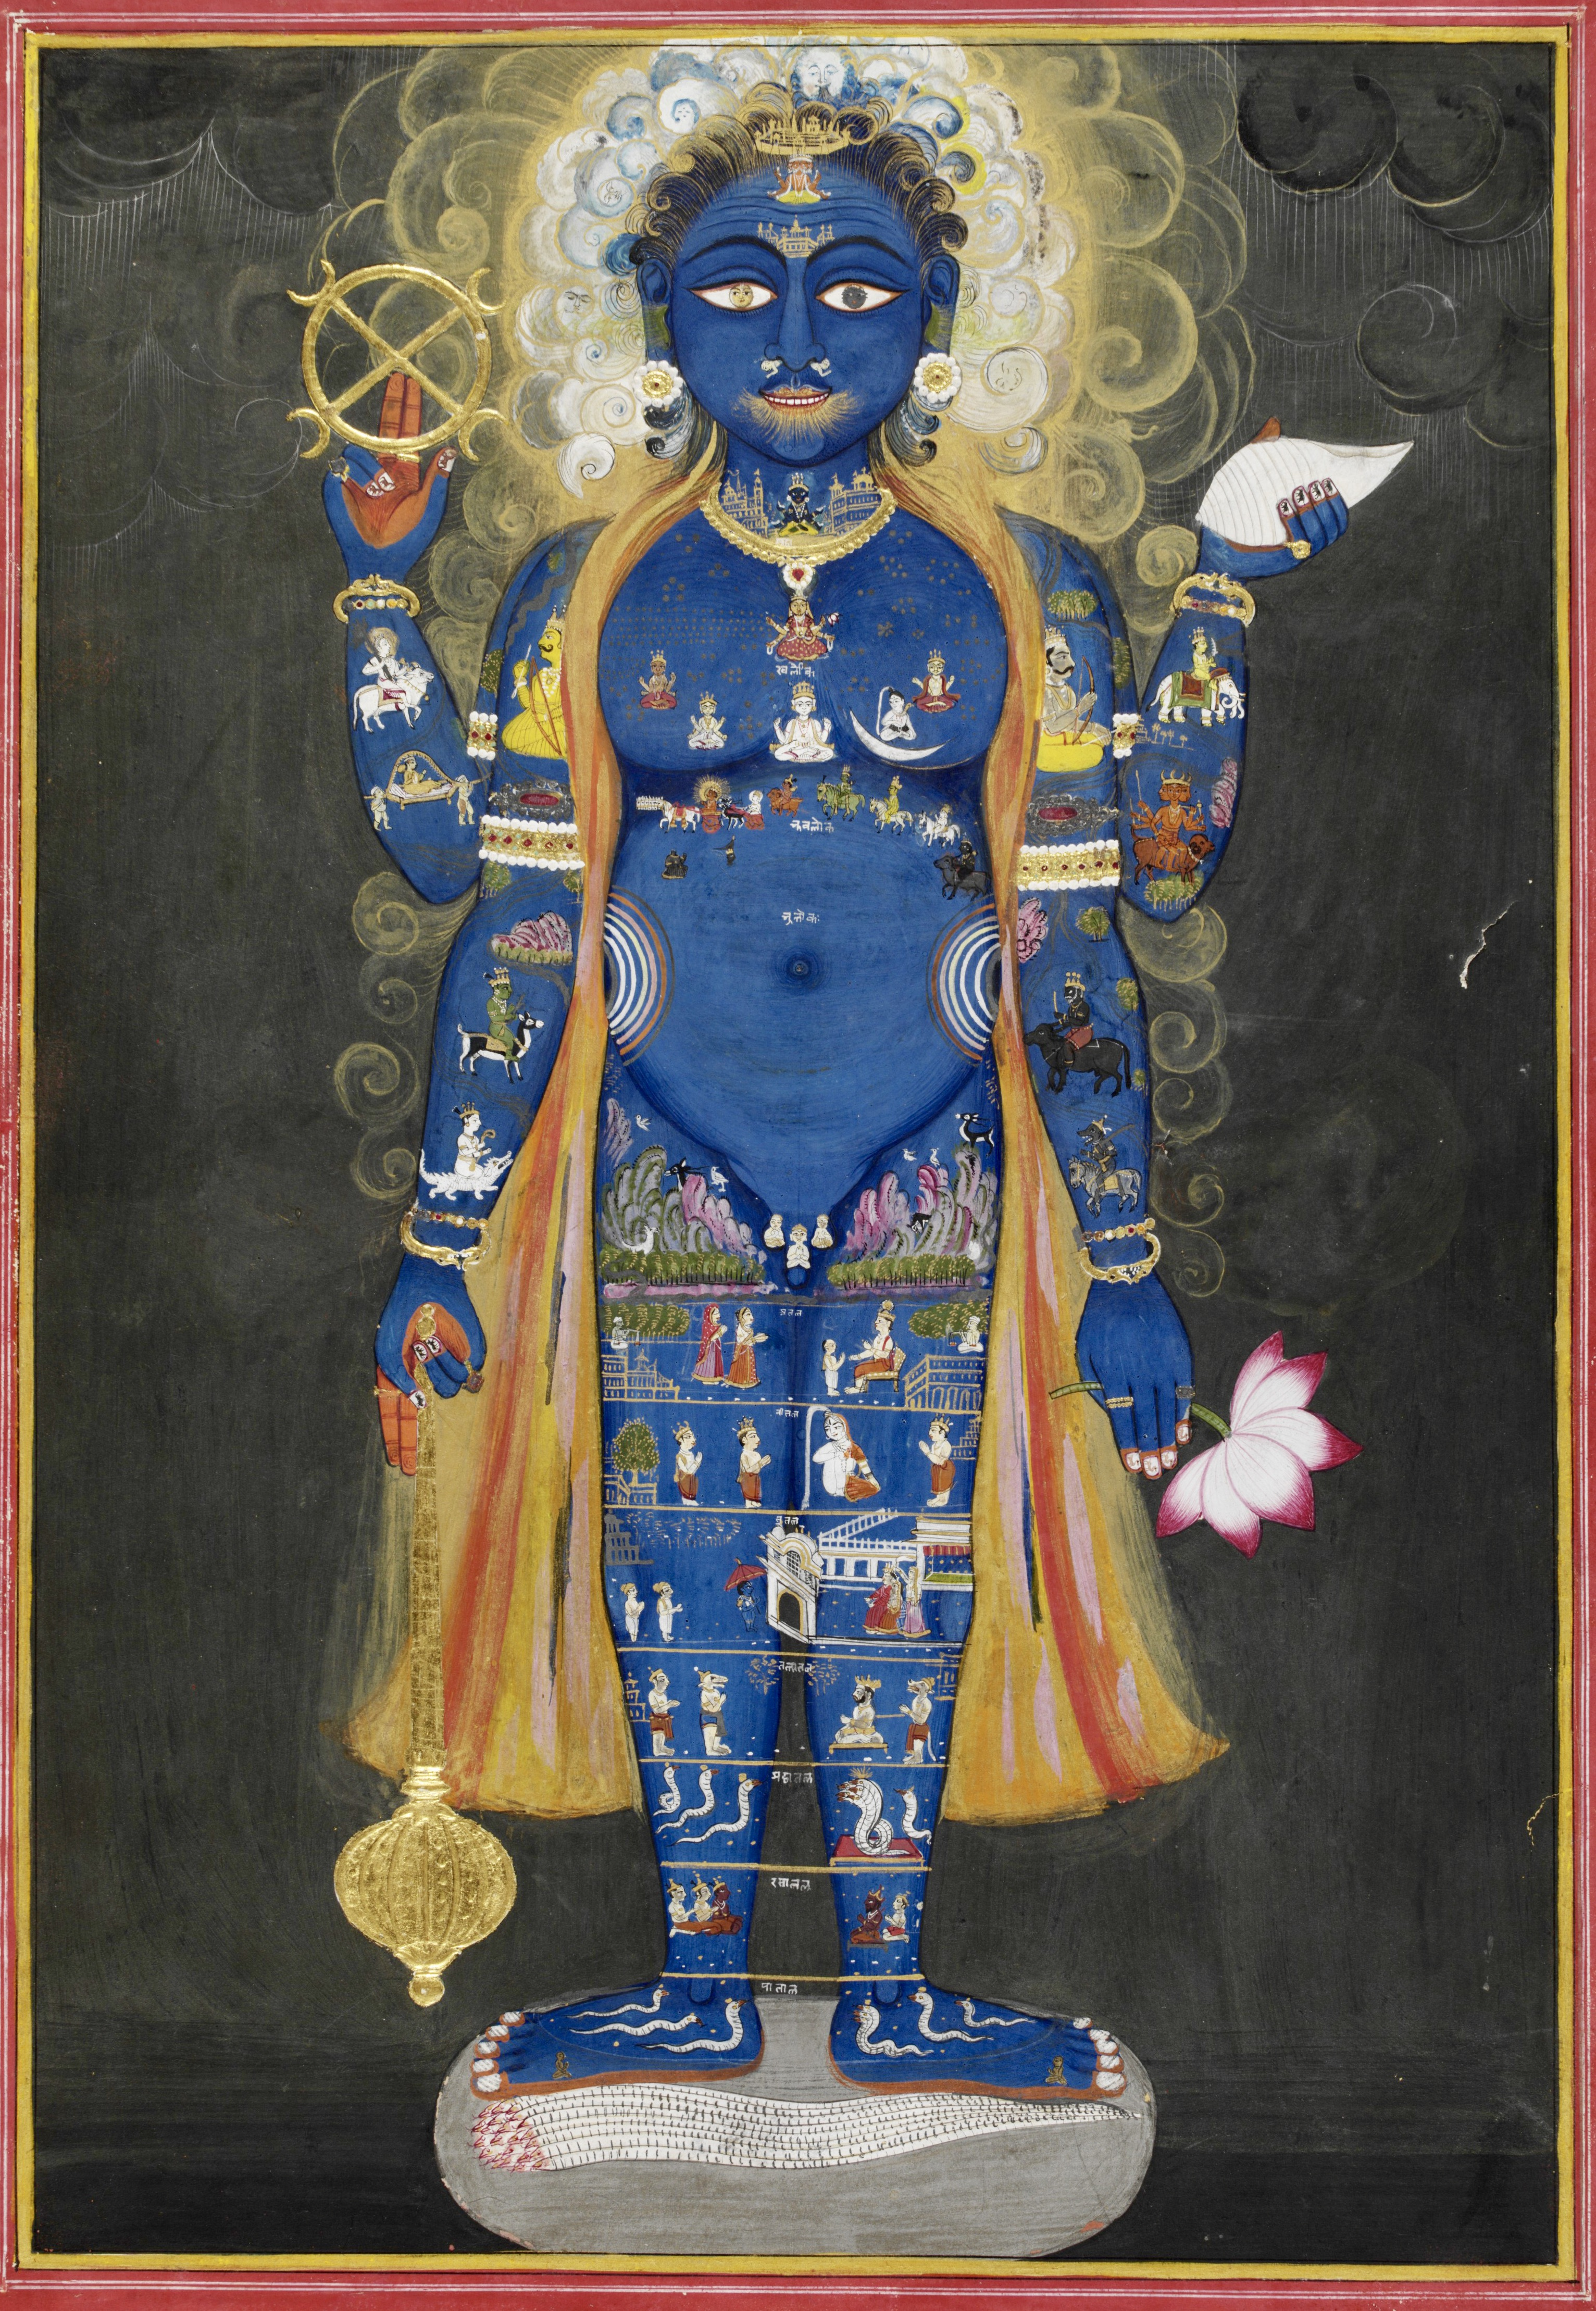
\includegraphics[width=1\textwidth]{pics/Vishnu_Vishvarupa_cropped.jpg}
	\caption{Viṣṇu Viśvarūpa, India, Rajasthan, Jaipur, ca. 1800–1820, Opaque watercolor and gold on paper, 38.5 × 28 cm, Victoria and Albert Museum, London, Given by Mrs. Gerald Clark.}
	\label{fig1}
      \end{figure}
\clearpage
  \begin{figure}[ht]
	\centering
  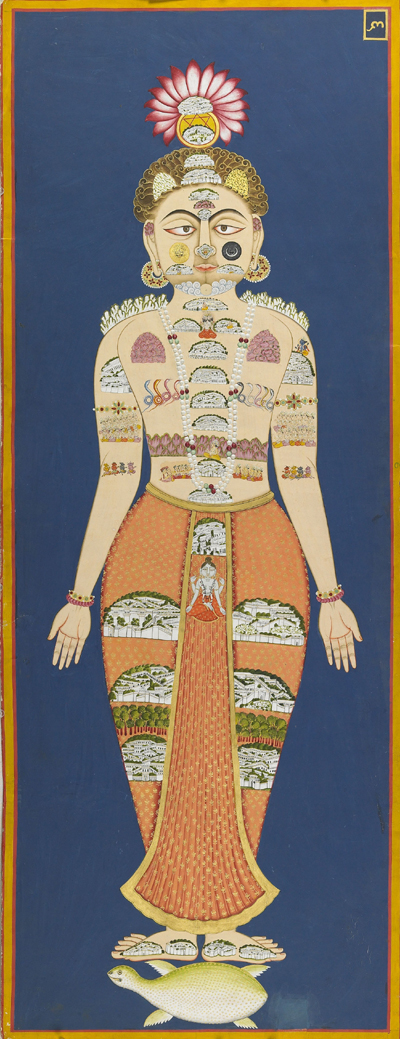
\includegraphics[width=0.5\textwidth]{pics/The_Equivalence_of_Self_and_Universe_(detail),_folio_6_from_the_Siddha_Siddhanta_Paddhati,_(Bulaki),_1824_(Samvat_1881);_122_x_46_cm._Mehrangarh_Museum_Trust..jpg}
	\caption{The Equivalence of Self and Universe (detail), folio 6 from the \textit{Siddhasiddhāntapaddhati} (Bulaki), India, Rajasthan, Jodhpur, 1824 (Samvat 1881), 122 x 46 cm, RJS 2378, Mehragarh Museum Trust.}
	\label{fig2}
      \end{figure}
      % \end{landscape}


\chapter{Bibliography}
 \label{sec:bibli}
   \clearpage
\newpage 
\thispagestyle{empty}
\quad  \addtocounter{page}{-1}

\printbibliography[heading=subbibintoc, title=Consulted Manuscripts, keyword=codex]

\printbibliography[heading=subbibintoc, title=Printed Editions, keyword=printsource]

\printbibliography[heading=subbibintoc, title=Secondary Literature, keyword=seclit]

\printbibliography[heading=subbibintoc, title=Online Sources, keyword=onlinesource]

\end{document}
